\documentclass[a4paper]{article}

%% Language and font encodings
\usepackage[english]{babel}
\usepackage[utf8x]{inputenc}
\usepackage[T1]{fontenc}

%% Sets page size and margins
\usepackage[a4paper,top=3cm,bottom=2cm,left=3cm,right=3cm,marginparwidth=1.75cm]{geometry}

%% Useful packages
\usepackage{amsmath}
\usepackage{graphicx}
\usepackage[colorinlistoftodos]{todonotes}
\usepackage[colorlinks=true, allcolors=blue]{hyperref}
\usepackage{algorithm}
\usepackage{algorithmic}
\usepackage{verbatim}
\usepackage{arev}
\usepackage{txfonts}

\title{Graduate Preliminary Exam: Spring 2014}
\author{Zhengyang Song}

\begin{document}
\maketitle

\section{Longest path in a DAG}

We are given a directed acyclic graph $G$ and two specific vertices $s$ and $t$ in $G$. Each edge in the graph has a length. Design a polynomial time algorithm that finds the longest path from $s$ to $t$. (if there is not path from $s$ to $t$, your algorithm should be able to detect the fact.)

\ \\{\bf Solution:} First do a topology sort in polynomial time. If $t$ is before $s$, return no path. We now only care about the edges between $s$ and $t$, discard all the others. 

Then run a DFS to enumerate the graph.


\section{Monge Matrix}
\[
A[i,j] + A[k,l] \le A[i,l]+A[k,j], \forall i<k\ \text{and}\ j<l
\]
\[\begin{pmatrix}
10 & 9 & 12 & 10\\
11 & 10 & 13 & 10\\
9 & 8 & 0 & 7\\
11 & 10 & 11 & 8
\end{pmatrix}\]
Let $f(i)$ be the column index of the leftmost minimum element of row $i$.
\begin{enumerate}
\item Show that $f(1)\le f(2)\le \dots\le f(m)$.
\item Given an $m\times n$ Monge matrix, design an algorithm that computes $f(1),\dots,f(m)$ in $O(m+n\log m)$ time.
\end{enumerate}
{\bf Solution:}
\begin{enumerate}
\item For $i < j$, we want to prove $f(i) \le f(j)$. Suppose otherwise, we have $f(i) = s > f(j) = t$. Then 
\[
A[i,s] < A[i,t]
\]
\[
A[j,t] \le A[j,s]
\]
\[
A[i,s] + A[j,t] < A[i,t] + A[j,s]
\]
It contradicts with the definition of Monge matrix.
\item We use divide-and-conquer. We first find $f(\lfloor m/2\rfloor)$ in time $O(n)$. Then based on the above conclusion, we can safely drop the bottom left quarter and top right quarter. Do the same operation for the top left quarter and bottom right quarter. Note that this procedure will end in $O(\log m)$ rounds. In each round, the total time cost for all the subtasks are $O(n)$. Furthermore, output all the results will cost time $O(m)$. That leads us to the time complexity of $O(m+ n\log m)$.
\end{enumerate}


\section{}

An interval graph is undirected graph $G=(V,E)$ where vertices correspond to intervals on the real line, where each interval is specified by a leftmost value $v_1$ and a rightmost value $v_2$. Two vertices in $G$ are connected iff the corresponding intervals overlap. Let $G$ be an interval graph whose corresponding intervals are provided. Give a polynomial time algorithm to find a maximum independent set in $G$. You need to prove the correctness of your algorithm. (An independent set in a graph is a subset of vertices such that no two vertices in the subset are joined by an edge.)

\ \\{\bf Solution:} This problem is equivalent to find the maximum set of intervals with no intersection. We can use greedy algorithm. First sort the intervals using the rightmost value as key. Then go through the sorted list, each time we select the interval with the minimal rightmost value that has no intersection with the already selected ones. We show the correctness as follows.

Suppose there is another set of intervals $S'$ that is different from the result of our algorithm $S$. Then after sorting $S'$, we can always find the first interval $i'$ in $S'$ that is different from $i$ in $S$. We simply replace $i'$ with $i$, note that this will not violent the independent property. We can always do this until the last element of $S'$. Thus we have $|S'| \le |S|$


\section{}

Show that finding a min-cost matching with exactly $k$ edges in a bipartite graph $G(U,V;E)$ (with positive edges) can be solved in polynomial time. Note that $|U|$ may not be the same as $|V|$. You can assume that the min-cost perfect matching problem in a bipartite graph can be solved in polynomial time.

\ \\{\bf Solution:} We can turn this into a minimum-cost maximum-flow probelm. Add a source $s$ and a sink $t$, together with a $s'$ and $t'$, where there is an edge with capacity $k$ from $s$ to $s'$, and an edge with capacity 1 from $s'$ to all the vertices in $U$. The same is with $t'$ and $t$. The edges in $E$ are all assigned with a capacity 1. All newly added edges are assigned with a cost 0. Then we just need to compute the minimum-cost maximum-flow of this new graph $G'$, where a polynomial algorithm exists.


\section{Finding the maximum area polygon}

\ \\{\bf Solution:} We can use a dynamic programming method. Suppose the polygon is rooted at 0, then we let $dp[m][i]$ be the maximum area we can get for a $m$-gon with the largest index vertex $i$. 
\[
dp[m][i] = max(\{dp[m-1][j]+area(0, i, j)|j<i\})
\]
Then the answer for root 0 is just
\[
answer = max(\{dp[n][i] | 1\le i\le n\}) 
\]
Then we enumerate all the possible root position (rather than 0) in time $O(n)$. That completes our polynomial algorithm.
\section{Edit distance}

In order to transform one string x to a target string y,we can perform various edit operations. Our goal is,given x and y,to produce a series of edits that change x to y. We may choose from among edit operations:
\begin{itemize}
\item Insert a letter, (e.g., changing 100 to 1001 takes one insertion) 
\item Delete a letter, (e.g., changing 100 to 10 takes one deletion) 
\item Replace a letter by another (e.g., you need do one replacement to change 100 to 000).
\end{itemize}
Design an efficient algorithm that finds a series of edit operations that change x to y and the total number of edits is minimized. 

{\bf Solution:} Denote $dp[i][j]$ as the optimal number of operations to transform $x[:i]$ to $y[:j]$. Then we have
\[
dp[i][j] = dp[i-1][j-1], \text{if } x[i]=y[j]
\]
\[
dp[i][j] = 1+\min(dp[i][j-1], dp[i-1][j], dp[i-1][j-1]), \text{if } x[i]\ne y[j]
\]
\[
dp[i][j] = i, \text{if } j=0
\]
\[
dp[i][j] = j, \text{if } i=0
\]
The answer is just $dp[len(x)][len(y)]$.

\section{Probability theory and probabilistic reasoning}

\begin{enumerate}
\item 
\ {\bf Solution:}
\[
P(young|use) = \frac{P(young)P(use|young)}{P(use)} = \frac{0.8}{0.8+0.2+0.4\times2}
\]
\item A Bayesian Network is a DAG to represent the conditional dependencies for a set of random variable. Given $n$ random variables, how many possible Bayesian Networks could be constructed to represent their conditional dependencies?

\ \\{\bf Solution:} The question is how many different DAGs can be formed using $n$ nodes. % http://arantxa.ii.uam.es/~ssantini/writing/notes/s649_dag_counting.pdf

\[
G(n)=\sum_{m=1}^n \sum_{n_1+\dots+n_m=m,n_i\ge1} \prod_{i=1}^{m-1} (2^{[i]}-2^{[i-1]})^{n_{i+1}}
\]
where $[k]=\sum_{h=1}^k n_h$

\item {\bf Solution:} No. Since D is dependent on C, and C is dependent on A. Image $P(C=true|A=true)=1$ and $P(D=true|C=ture)=1$, then $P(D=true|A=true) = 1$. The fact that no edge from A to D only means that A does not directly influence D.

\begin{eqnarray*}
P(E|A) &=& P(B|A) P(C|A,B) P(E|C)
\end{eqnarray*}

\item Are small Markov blankets better when performing inference using Gibbs sampling? Briefly explain in one or two sentences why or why not.

\ \\{\bf Solution:} Yes. Because when Markov blanket is large, the inference won't change much.
\end{enumerate}

\section{General machine learning}

\begin{enumerate}
\item In the curve fitting problem on a set of data points, what is the disadvantage of Nearest Neighbors approach compared to Least Squares method?

\ \\{\bf Solution:} Every time we need to start the computation from zero. It is computationally expensive to find the k nearest neighbors when the dataset is very large. Performance depends on the number of dimensions that we have.

On the other hand, it is important how we compute the distance (there may be unrelated features). Also when the dimension is large, the sample data tends to be located at the corner, causing the distance metric meaningless. One solution is to use weighed features to compute the distance. (Credit to Tianqi Zhao) 

\item True/False ``When training a linear regression estimator, 10-fold cross-validation has smaller bias than 5-fold cross-validation''

\ \\{\bf Solution:} Yes. Bias is different from variance. The model we train as a part of the testing procedure, would be as close as possible to the one that we would get if we trained it on the entire dataset.
\end{enumerate}

\section{Maximum Likelihood (ML)}

\begin{enumerate}
\item 
\[
L(\theta) = \theta\cdot 3\theta\cdot (1-3\theta)\cdot (1-3\theta) = 3\theta^2(3\theta-1)^2
\]
\item 
\[ L(\theta) = \frac{1}{3} (3\theta(1-3\theta))^2 \le \frac{1}{3} (\frac{3\theta+1-3\theta}{2})^4 = \frac{1}{48}
\]
where the equation sign is when
\[
3\theta = 1-3\theta \Rightarrow \theta = \frac{1}{6}
\]
\end{enumerate}

\section{Stick Game}
{\bf Solution:} We just maintain a bool array $win[i]$, which means if there are $i$ sticks left, then the next player will win. Then we show how to compute $win[n]$ in polynomail time.

We initialize 
\[
win[0]=false, win[1]=true, win[2]=false, win[3]=true, win[4]=true
\]

Then the recursion is as 
\[
win[i] = true \text{ if } win[i-1] = false \text{ or } win[i-4]=false
\]
\[
win[i] = false \text{ if } win[i-1] = true \text{ and } win[i-4] = true
\]
\section{Mongo Matrix}
\[
A[i,j] + A[k,l] \le A[i,l]+A[k,j], \forall i<k\ \text{and}\ j<l
\]
\[\begin{pmatrix}
10 & 9 & 12 & 10\\
11 & 10 & 13 & 10\\
9 & 8 & 0 & 7\\
11 & 10 & 11 & 8
\end{pmatrix}\]
Let $f(i)$ be the column index of the leftmost minimum element of row $i$.
\begin{enumerate}
\item Show that $f(1)\le f(2)\le \dots\le f(m)$.
\item Given an $m\times n$ Monge matrix, design an algorithm that computes $f(1),\dots,f(m)$ in $O(m+n\log m)$ time.
\end{enumerate}
{\bf Solution:}
\begin{enumerate}
\item For $i < j$, we want to prove $f(i) \le f(j)$. Suppose otherwise, we have $f(i) = s > f(j) = t$. Then 
\[
A[i,s] < A[i,t]
\]
\[
A[j,t] \le A[j,s]
\]
\[
A[i,s] + A[j,t] < A[i,t] + A[j,s]
\]
It contradicts with the definition of Monge matrix.
\item We use divide-and-conquer. We first find $f(\lfloor m/2\rfloor)$ in time $O(n)$. Then besed on the above conclusion, we can safely drop the bottom left quarter and top right quarter. Do the same operation for the top left quarter and bottom right quarter. Note that this procedure will end in $O(\log m)$ rounds. In each round, the total time cost for all the subtasks are $O(n)$. Furthermore, output all the results will cost time $O(m)$. That leads us to the time complexity of $O(m+ n\log m)$.
\end{enumerate}


\section{Cross-Validation}

What is the advantage of using a larger value, e.g. $k=10$, rather than e.g. $k=2$? Is there any advantage of using $k=2$ rather than $k=10$?

{\bf Solution:} A larger k will introduce smaller bias, while a larger variance. 

\section{Clustering}

\begin{enumerate}
\item Which of the two choices Single Linkage or Complete Linkage clustering will typically result in clusters with a small diameter? Why?

\ \\{\bf Solution:} In single-link clustering or single-linkage clustering , the similarity of two clusters is the similarity of their most similar members. In complete-link clustering or complete-linkage clustering , the similarity of two clusters is the similarity of their most dissimilar members.

Complete Linkage. Since in Single Linkage clustering, more distant parts of the cluster and the clusters' overall structure are not taken into account

\item The algorithm's output can be visualized using a dendrogram. Explain in one or two sentences if there are any disadvantages of dendrograms on this dataset.

\ \\{\bf Solution:} The dendrograms may be complex, and the horizontal split line may be hard to recognize.

\item Explain in one or two sentences if there would be any advantage of instead using the k-means algorithm on this dataset.

\ \\{\bf Solution:} The time complexity and space complexity is lower.

\end{enumerate}

\section{SVM}

\[
\begin{matrix}
x_{i1} & x_{i2} & y_i & \alpha_i \\
1 & 4 & 1 & 2\\
1.5 & 7 & 1 & 0\\
2 & 6 & 1 & 0\\
\end{matrix}
\]
\begin{enumerate}
\item What are the support vectors of this training data?

\ \\{\bf Solution:} where the $\alpha_i\ne 0$.

\item Assume that the decision surface bias is $b=-1.8$. Compute the weight vector $w$ using the data in the table given above.

\ \\{\bf Solution:} 
\[ 
w = \sum \alpha_i x_iy_i
\]

\item Consider the points $(1,4),(4.5,3),(2,2)$ and $(3,1)$ from the table above. How are these points classified by the model? Compute the slack variables $x_i$ for these points.

\item Use the SVM model to compute a classification for a test data point $(4,4)$.

\ \\{\bf Solution:}
\[
y = w^Tx+b
\]
\end{enumerate}

\section{Perceptron and Kernel Methods}
\begin{enumerate}
\item Does the Perceptron algorithm have any advantages over the regular SVM algorithm?

\ \\{\bf Solution:} Perceptrons can be trained online (i.e. their weights can be updated as new examples arrive one at a time).
\[
w \leftarrow w + y_ix_i
\]

\item Under what circumstance can a machine learning algorithm be kernelized (i.e, adapted to work with kernels)? Can you find a way to do this for the Perceptron algorithm? Explain the changes you need to make to it and why these changes are acceptable. Also explain whether this algorithm has any disadvantages.

\ \\{\bf Solution:}
\[
w \cdot x + b = \sum_{j\in E} y_j x_j \cdot x + b
\]
\end{enumerate}

We need to find a good kernel function.


\section{Graphical Models}

In this MRF model, the associated potential functions are defined by 
\[
\phi(x,y)=2xy+x^3
\]
\[
\phi(x,z)=xz+z
\]
\[
\phi(y,z)=yz^3
\]

\begin{enumerate}
\item Compute the posterior marginal probability $P(y|x=1)$

\ \\{\bf Solution:} 
\[
P(x,y,z) = \frac{1}{Z} \prod \phi(x,y)\phi(y,z)\phi(x,z) 
\]
\begin{eqnarray*}
Z &=& \sum\prod \phi(x,y)\phi(y,z)\phi(x,z) \\
&=& (2+1)(1+1)(1) + \cdots
\end{eqnarray*}
Note: actually we do not need to compute $Z$ explicitly, since it will be cancelled out in later calculation. (Credit to Xin Liu $\varheartsuit$)
\[
P(x,y) = \sum_z P(x,y,z)
\]
\[
P(x) = \sum_{y,z} P(x,y,z)
\]
\[
P(y|x=1) = \frac{P(x=1,y)}{P(x=1)}
\]

\item In the following three directed graphical models, assume variable $y$ has been observed:
\[
x\rightarrow y\rightarrow z
\]
\[
x\rightarrow y\leftarrow z
\]
\[
x\leftarrow y \rightarrow z
\]
In the above three directed models, argue whether $x$ and $z$ are conditionally independent, given $y$. 

\ \\{\bf Solution:} 
Independent:
\[
P(x,z|y) = \frac{P(x,z,y)}{P(y)} = \frac{P(x)P(y|x)P(z|y)}{P(y)} = P(x|y)P(z|y)
\]
Not independent:
\[
P(x,z|y) = \frac{P(x,y,z)}{P(y)} = \frac{P(x)P(z)P(y|x,z)}{P(y)}\ne P(x|y) P(z|y)
\]
Independent:
\[
P(x,z|y) = \frac{P(x,y,z)}{P(y)} = \frac{P(y)P(x|y)P(z|y)}{P(y)} = P(x|y) P(z|y)
\]
\end{enumerate}

\section{Ensemble learning}

Write a rigorous derivation showing that that bagging decreases the mean squared error rate of a regression task, compared to the single regressor trained on $D$.

\ \\{\bf Solution:} PRML P656.

\section{Hidden Markov model}

We can model $p(x_1^T)=\sum_{s_1^T}\prod_{t=1}^Tp(x_t,s_t|x_1^{t-1},s_1^{t-1})$.
\begin{enumerate}
\item Write down the model for $p(x_1^T)$ using dependencies only on the previous state (first-order Markov)
\item Write a generalized Hidden Markov Model that employs the forward algorithm for scoring.
\item What is the time complexity of the algorithm in direct calculation of (1) and forward algorithm of (2).
\end{enumerate}


\section{EM}

Explain and prove the convergence of EM algorithm.

\ \\{\bf Solution:} 
\begin{itemize}
\item Expected complete data log likelihood is a lower bound. 
\item EM monotonically increases the observed data log likelihood.
\end{itemize}

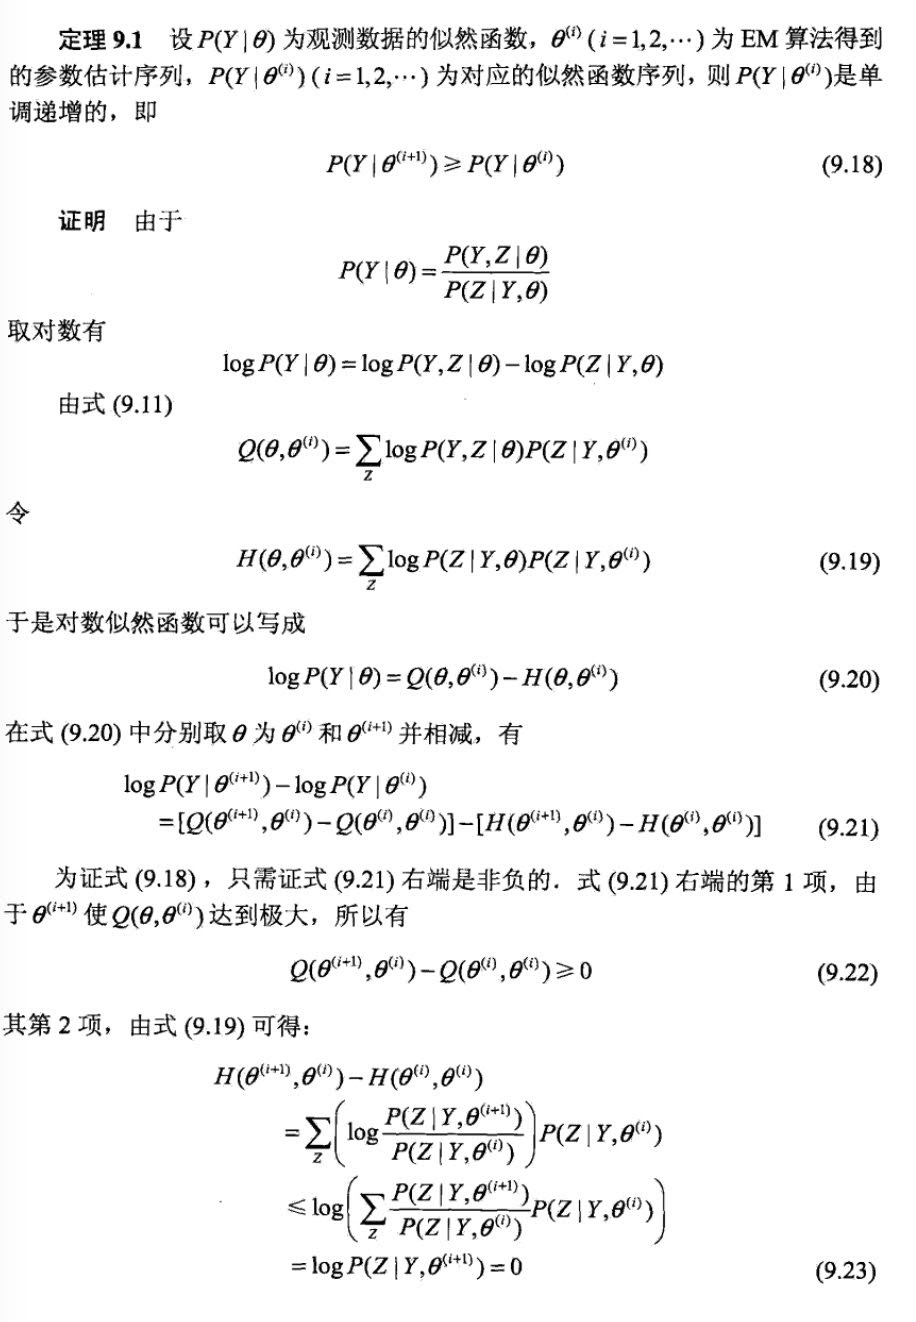
\includegraphics[width=\columnwidth]{19}

\end{document}